\documentclass[9pt]{osa-supplemental-document}
\setboolean{shortarticle}{false}

\usepackage{booktabs}

\newcommand{\chitwo}{\chi^{(2)}}
\newcommand{\chithree}{\chi^{(3)}}
\newcommand{\chicasc}{\chi^{(3)}_{\mathrm{casc}}}
\newcommand{\chinat}{\chi^{(3)}_{\mathrm{nat}}}
\newcommand{\Dom}{\Delta\omega}
\newcommand{\etag}{\eta_{\mathrm{geom}}}
\newcommand{\f}{\mathbf f}
\newcommand{\h}{\mathbf h}
\newcommand{\acasc}{\alpha_{\mathrm{casc}}}
\newcommand{\NL}{\mathrm{NL}}
\newcommand{\figbox}[1]{%
  \fbox{\parbox[c][#1][c]{0.9\linewidth}{\centering\small figure in preparation}}}

\title{Resonant cascaded Kerr nonlinearity in $\chi^{(2)}$ metasurfaces: supplemental document}
\author{}

\begin{abstract}
Derivation of the cascaded susceptibility of a resonator, its uniform-medium
limit, its frequency response and strength--bandwidth relation, the
thresholds, the host-material parameters, the coupled-mode simulations, the
singly resonant metasurface and the microring model.
\end{abstract}

\setboolean{displaycopyright}{false}

\begin{document}

\maketitle

\section{Coupled-mode equations and the cascaded susceptibility}

\subsection{Conventions and modes}

Real fields are written as $\mathcal E=\mathbf E e^{-i\omega t}+\mathrm{c.c.}$
without a factor $\tfrac12$, so that the time average of $\mathcal E^2$ is
$2|\mathbf E|^2$.  With $\mathbf E_1$ and $\mathbf E_2$ the complex amplitudes
at $\omega_1$ and $2\omega_1$, the second-harmonic, difference-frequency and
self-phase-modulation polarisations are~\cite{boyd2020}
\begin{equation}
  P_i(2\omega_1)=\varepsilon_0\chitwo_{ijk}E_{1,j}E_{1,k},\quad
  P_i(\omega_1)=2\varepsilon_0\chitwo_{ijk}E_{2,j}E^*_{1,k},\quad
  P_i(\omega_1)=3\varepsilon_0\chithree_{ijkl}E_{1,j}E_{1,k}E^*_{1,l},
  \label{eq:pol}
\end{equation}
where the factors 2 and 3 count the distinct orderings of the input
frequencies.  Kleinman symmetry makes $\chitwo_{ijk}$ invariant under
permutation of its indices, so one real tensor $\chitwo_{ijk}(\mathbf r)$
describes both second-order processes.

Mode $n$ has the resonance frequency $\bar\omega_n$, with
$\bar\omega_1=\omega_a$ for the pump mode and $\bar\omega_2=\omega_2$ for
the second-harmonic mode, and satisfies
$\nabla\times\nabla\times\f_n=(\bar\omega_n^2/c^2)\varepsilon_r(\mathbf r,\bar\omega_n)\f_n$
with $\h_n=-i\nabla\times\f_n/(\mu_0\bar\omega_n)$.  We define
\begin{equation}
  N_n=\frac12\int\bigl(\varepsilon_0\tilde\varepsilon_n|\f_n|^2+\mu_0|\h_n|^2\bigr)d^3r,
  \qquad
  \tilde\varepsilon_n=\left.\frac{\partial(\omega\varepsilon_r)}{\partial\omega}\right|_{\bar\omega_n},
  \label{eq:Nn}
\end{equation}
so that, by Brillouin's expression for the energy in a dispersive medium,
the field $a_n\f_ne^{-i\bar\omega_nt}+\mathrm{c.c.}$ stores the energy
$W_n=2N_n|a_n|^2$.  For an eigenmode
$\int\varepsilon_0\varepsilon_r|\f_n|^2d^3r=\int\mu_0|\h_n|^2d^3r$, and
$N_n=\int\varepsilon_0\varepsilon_r|\f_n|^2d^3r$ in a nondispersive
medium.  The susceptibilities and overlaps below do not depend on the
normalisation of the modes.

\subsection{Projection onto a mode}

Write the field near frequency $\omega$ as
$\mathcal E=a(t)\f_n(\mathbf r)e^{-i\omega t}+\mathrm{c.c.}$ with a slowly
varying amplitude $a$, and the nonlinear polarisation in the same band as
$\mathbf Pe^{-i\omega t}$ plus its complex conjugate.  The
positive-frequency part of
$\nabla\times\nabla\times\mathcal E+c^{-2}\partial_t^2\mathcal D_{\mathrm{lin}}/\varepsilon_0=-\mu_0\partial_t^2\mathcal P$,
where $\mathcal D_{\mathrm{lin}}$ is the linear displacement field and
$\mathcal P$ the nonlinear polarisation, contains the operator $(\omega+i\partial_t)^2\varepsilon_r(\omega+i\partial_t)$.
To first order in $\partial_t$ and in $\omega-\bar\omega_n$ it equals
$\bar\omega_n^2\varepsilon_r(\bar\omega_n)-\bar\omega_n(\varepsilon_r+\tilde\varepsilon_n)(\bar\omega_n-\omega)+i\bar\omega_n(\varepsilon_r+\tilde\varepsilon_n)\partial_t$.
Neglecting $\dot{\mathbf P}$ against $\omega\mathbf P$ and projecting onto
$\f_n^*$ gives
\begin{equation}
  \dot a=i(\omega-\bar\omega_n)\,a+\frac{i\omega}{2N_n}\int\f_n^*\cdot\mathbf P\,d^3r ,
  \label{eq:projection}
\end{equation}
since $\int\varepsilon_0(\varepsilon_r+\tilde\varepsilon_n)|\f_n|^2d^3r=2N_n$.
For a static perturbation in a nondispersive medium this is the
first-order frequency shift
$-(\bar\omega_n/2)\int\mathbf E^*\cdot\delta\mathbf P\,d^3r/\int\varepsilon_0\varepsilon_r|\mathbf E|^2d^3r$~\cite{johnson2002}.
Radiation and absorption are included by giving $\bar\omega_n$ the
imaginary part $-\gamma_n/2$, and the pump detuning is
$\delta_1=\omega_1-\omega_a$.  The pump mode is driven by the term
$(\gamma_1^{\mathrm e}/2N_1)^{1/2}s$, where $|s|^2$ is the incident power
and $\gamma_1^{\mathrm e}$ is
the decay rate into the channel of the incident wave, half the radiative
rate for a structure that radiates equally to both sides.

\subsection{Coupling constants}

With $\mathbf E_1=a_1\f_1$ and $\mathbf E_2=a_2\f_2$, the three sources of
Eq.~\eqref{eq:pol} give, through Eq.~\eqref{eq:projection},
\begin{align}
  \int\f_2^*\cdot\mathbf P(2\omega_1)\,d^3r&=\varepsilon_0Ma_1^2,
  &\beta&=\frac{\varepsilon_0\omega_1M}{N_2},\\
  \int\f_1^*\cdot\mathbf P_{\mathrm{DFG}}(\omega_1)\,d^3r&=2\varepsilon_0M^*a_1^*a_2,
  &\beta_1&=\frac{\varepsilon_0\omega_1M}{N_1},\\
  \int\f_1^*\cdot\mathbf P_{\mathrm{SPM}}(\omega_1)\,d^3r&=3\varepsilon_0K|a_1|^2a_1,
  &\alpha_3&=\frac{3\varepsilon_0\omega_1}{2N_1}K,
\end{align}
with $M=\int\chitwo_{ijk}f^*_{2,i}f_{1,j}f_{1,k}\,d^3r$ and
$K=\int\chithree_{ijkl}f^*_{1,i}f_{1,j}f_{1,k}f^*_{1,l}\,d^3r$.  The second
line uses Kleinman symmetry,
$\int\chitwo_{ijk}f^*_{1,i}f_{2,j}f^*_{1,k}\,d^3r=M^*$.  These are the
coefficients of Eqs.~(1) and (2) of the main text.  In the absence of loss
and drive,
\begin{equation}
  \frac{d}{dt}\bigl(N_1|a_1|^2+N_2|a_2|^2\bigr)
  =-2\,\mathrm{Im}\bigl(\varepsilon_0\omega_1M^*a_1^{*2}a_2\bigr)
   +2\,\mathrm{Im}\bigl(\varepsilon_0\omega_1M^*a_1^{*2}a_2\bigr)=0 ,
\end{equation}
so the stored energy $W_1+W_2$ is conserved, which requires the factor 2
of the difference-frequency polarisation.

\subsection{Steady-state elimination}

If $a_1^2$ varies slowly on the time scale $|\Dom+i\gamma_2/2|^{-1}$,
Eq.~(2) of the main text gives $a_2=-\beta a_1^2/(\Dom+i\gamma_2/2)$ with
$\Dom=2\omega_1-\omega_2$.  The term $i\beta_1^*a_1^*a_2$ of Eq.~(1) of the
main text becomes $i\acasc|a_1|^2a_1$ with
\begin{equation}
  \acasc=-\frac{\beta_1^*\beta}{\Dom+i\gamma_2/2}
  =-\frac{\varepsilon_0^2\omega_1^2|M|^2}{N_1N_2(\Dom+i\gamma_2/2)} .
  \label{eq:acasc}
\end{equation}
Integration of the two-mode equations reproduces Eq.~\eqref{eq:acasc}
[Fig.~\ref{fig:s-checks}(a)].  The real part of $\acasc$ shifts the pump
resonance, and its imaginary part,
\begin{equation}
  \mathrm{Im}\,\acasc=\frac{\varepsilon_0^2\omega_1^2|M|^2\,\gamma_2/2}{N_1N_2[\Dom^2+(\gamma_2/2)^2]},
\end{equation}
reduces the pump energy at the rate $2\,\mathrm{Im}\,\acasc|a_1|^2W_1$,
which in steady state equals the power $\gamma_2W_2$ lost by the
second-harmonic mode.

The native susceptibility $\chinat$ of the second-order material is
defined by $K=\chinat\int_{\NL}|\f_1|^4d^3r$, so that
\begin{equation}
  \alpha_3=\frac{3\varepsilon_0\omega_1}{2N_1}\,\chinat\int_{\NL}|\f_1|^4d^3r ,
\end{equation}
where $\int_{\NL}$ extends over that material.  For an isotropic response
and a mode that is linearly polarised everywhere in the material,
$\chinat=\chithree_{xxxx}$.  Other materials in the cell are assumed to
have a negligible $\chithree$, and the native response is taken to be
lossless.  Defining $\chicasc$ in the same way through $\acasc$ gives
\begin{equation}
  \chicasc=-\frac{2\varepsilon_0\omega_1}{3N_2}\,
  \frac{|M|^2}{(\Dom+i\gamma_2/2)\int_{\NL}|\f_1|^4d^3r},
  \label{eq:chicasc}
\end{equation}
in which $N_1$ cancels and $N_2$ cancels the normalisation of $\f_2$ in
$|M|^2$.  With the overlap
$\etag=\varepsilon_0n_2^2|M|^2/(|\chitwo|^2N_2\int_{\NL}|\f_1|^4d^3r)$,
Eq.~\eqref{eq:chicasc} takes the form of Eq.~(3) of the main text, and
$\acasc/\alpha_3=\chicasc/\chinat$.

\subsection{Bound on the overlap}

Let $|\chitwo|$ be the largest value of $|\chitwo_{ijk}u^*_iv_jv_k|$ over
complex unit vectors $\mathbf u,\mathbf v$ and positions in the material.
It equals $2d_{33}$ for LiNbO$_3$ and AlN and $(2/\sqrt3)\,2d_{14}$ for
zincblende crystals, where the maximum is reached for fields along
$[111]$.  Let $n_2^2$ be the smallest principal value of $\varepsilon_r$ of
the material at $2\omega_1$, which is $n_e^2$ for LiNbO$_3$.  The
Cauchy--Schwarz inequality gives
\begin{equation}
  |M|^2\le|\chitwo|^2\int_{\NL}|\f_2|^2d^3r\int_{\NL}|\f_1|^4d^3r .
\end{equation}
For normal dispersion $\tilde\varepsilon_2\ge\varepsilon_r$, so that
$N_2\ge\int\varepsilon_0\varepsilon_r|\f_2|^2d^3r\ge\varepsilon_0n_2^2\int_{\NL}|\f_2|^2d^3r$,
and therefore $\etag\le1$.  Equality requires that $\f_2$ vanish outside
the material, that $\chitwo_{ijk}f_{1,j}f_{1,k}$ be parallel to $\f_2$ with
a constant ratio and magnitude $|\chitwo||\f_1|^2$, and that
$\tilde\varepsilon_2=\varepsilon_r=n_2^2$ wherever $\f_2$ is nonzero.  The
uniform medium of Section~3 meets these conditions when dispersion within
the second-harmonic band is neglected.  When both fields are uniform in
the material and aligned with the maximising direction, $\etag$ is the
fraction of the electric energy of the second-harmonic mode that lies in
the material.

\section{Green's-function form of the cascade}

At leading order in the nonlinearity the second-harmonic field obeys
\begin{equation}
  \bigl[\nabla\times\nabla\times-k_0^2\varepsilon_r(\mathbf r,2\omega_1)\bigr]\mathbf E_2
  =k_0^2\,\chitwo\!:\!\mathbf E_1\mathbf E_1 ,
  \label{eq:shwave}
\end{equation}
with $k_0=2\omega_1/c$ the vacuum wavenumber at $2\omega_1$, so that
\begin{equation}
  E_{2,j}(\mathbf r)=k_0^2\int G_{jl}(\mathbf r,\mathbf r')\chitwo_{lmn}(\mathbf r')E_{1,m}(\mathbf r')E_{1,n}(\mathbf r')\,d^3r' ,
\end{equation}
with $G$ the Green's function of the operator on the left.  Inserting this
field into the difference-frequency polarisation of Eq.~\eqref{eq:pol} gives
\begin{equation}
  P_i^{\mathrm{casc}}(\mathbf r)=2\varepsilon_0k_0^2E^*_{1,k}(\mathbf r)
  \int\chitwo_{ijk}(\mathbf r)\,G_{jl}(\mathbf r,\mathbf r')\,\chitwo_{lmn}(\mathbf r')\,
  E_{1,m}(\mathbf r')E_{1,n}(\mathbf r')\,d^3r' .
  \label{eq:kernel}
\end{equation}
The polarisation at $\mathbf r$ depends on the pump field at every point
that the second-harmonic field connects to $\mathbf r$, so the cascade is
nonlocal.  In a homogeneous crystal of length $L$ with $|\Delta k|L\gg1$
the kernel reduces to the local bulk response of Section~3.

Near an isolated mode the Green's function is dominated by its pole.
Expanding the operator of Eq.~\eqref{eq:shwave} about $\omega_2$ as in
Section~1.B gives
\begin{equation}
  G_{jl}(\mathbf r,\mathbf r';2\omega_1)\simeq
  -\frac{\varepsilon_0c^2}{4\omega_1N_2}\,
  \frac{f_{2,j}(\mathbf r)\,f^*_{2,l}(\mathbf r')}{\Dom+i\gamma_2/2}
  +G^{\mathrm{bg}}_{jl},
  \label{eq:pole}
\end{equation}
with a nonresonant background $G^{\mathrm{bg}}$.  For a leaky mode the
product $f_{2,j}f^*_{2,l}/N_2$ is replaced by the quasinormal-mode residue,
which contains the unconjugated product of the mode with its reciprocal
partner and a complex normalisation~\cite{sauvan2013,lalanne2018}.  For a
standing-wave mode with $Q_2=\omega_2/\gamma_2\gg1$ the field can be taken real inside the
resonator and the residue reduces to Eq.~\eqref{eq:pole}; the imaginary part
of the normalisation adds a correction of order $1/Q_2$ that makes the
response asymmetric about $\Dom=0$.  With $\mathbf E_1=a_1\f_1$,
Eq.~\eqref{eq:pole} gives $\mathbf E_2=a_2\f_2$ with
$a_2=-\beta a_1^2/(\Dom+i\gamma_2/2)$, the steady state of Eq.~(2) of the
main text, and Eq.~\eqref{eq:kernel} becomes
\begin{equation}
  P_i^{\mathrm{casc}}=-\frac{2\varepsilon_0^2\omega_1M|a_1|^2a_1}{N_2(\Dom+i\gamma_2/2)}\,
  \chitwo_{ijk}f_{2,j}f^*_{1,k}.
\end{equation}
Its projection onto $\f_1^*$ is
$-2\varepsilon_0^2\omega_1|M|^2|a_1|^2a_1/[N_2(\Dom+i\gamma_2/2)]$.
Equating it to the projection
$3\varepsilon_0\chicasc|a_1|^2a_1\int_{\NL}|\f_1|^4d^3r$ of a native
polarisation returns Eq.~\eqref{eq:chicasc}.

\section{Uniform-medium limit and a layered-cell test}

In a uniform isotropic medium with refractive indices $n_1$ at $\omega_1$
and $n_2$ at $2\omega_1$, a pump plane wave $A\hat{\mathbf x}e^{ik_1z}$ with
$k_1=n_1\omega_1/c$ drives the source $\varepsilon_0A^2\mathbf pe^{2ik_1z}$,
where $p_m=\chitwo_{mxx}$.  For the transverse part of $\mathbf p$,
Eq.~\eqref{eq:shwave} gives the bound wave
\begin{equation}
  \mathbf E_{2\perp}=\frac{\mathbf p_\perp A^2}{n_1^2-n_2^2}.
\end{equation}
For $\mathbf p_\perp=|\chitwo|\hat{\mathbf x}$ the difference-frequency
polarisation along $\hat{\mathbf x}$ is $2\varepsilon_0|\chitwo|E_{2,x}A^*$,
and
\begin{equation}
  \chi^{(3)}_{\mathrm{casc,bulk}}=-\frac{2|\chitwo|^2}{3(n_2^2-n_1^2)}
  \simeq-\frac{2\omega_1|\chitwo|^2}{3cn_2\Delta k},\qquad
  \Delta k=\frac{2\omega_1(n_2-n_1)}{c},
  \label{eq:bulk}
\end{equation}
where the second form holds to first order in $n_2-n_1$.  The longitudinal
component $p_z$ does not propagate, and $\nabla\cdot\mathbf D=0$ gives
$E_{2,z}=-p_zA^2/n_2^2$, which adds $-2p_z^2/(3n_2^2)$ to the cascaded
susceptibility.  This term does not depend on $\Dom$, is smaller than the
resonant one by a factor of order $|\Dom|/\omega_1$, and vanishes for a
transverse $\mathbf p$.

In a periodic box of volume $V$ filled with the medium, and neglecting
dispersion within the second-harmonic band,
$\f_1=\hat{\mathbf x}e^{ik_1z}/(\varepsilon_0n_1^2V)^{1/2}$ couples only to
$\f_2=\hat{\mathbf x}e^{2ik_1z}/(\varepsilon_0n_2^2V)^{1/2}$, whose
frequency is $\omega_2=2\omega_1n_1/n_2$, and $N_1=N_2=1$.  Then
$|M|^2=|\chitwo|^2/(\varepsilon_0^3n_1^4n_2^2V)$,
$\int|\f_1|^4d^3r=1/(\varepsilon_0^2n_1^4V)$, $\etag=1$, and
Eq.~\eqref{eq:chicasc} with $\Dom=2\omega_1(n_2-n_1)/n_2$ and $\gamma_2=0$
gives $-|\chitwo|^2/[3n_2(n_2-n_1)]$, which agrees with Eq.~\eqref{eq:bulk} to
first order in $n_2-n_1$.  The residual comes from linearising
$\omega_2^2-4\omega_1^2$ about the pole; with the full denominator of the
mode expansion the two expressions coincide.  Dispersion within the
second-harmonic band changes $N_2$ to $n_{g2}/n_2$ and $\Dom$ to
$c\Delta k/n_{g2}$, with $n_{g2}$ the group index at $2\omega_1$, so that
$\etag=n_2/n_{g2}$ and $\chicasc$ is unchanged.

To test Eq.~\eqref{eq:chicasc} in an inhomogeneous structure, we take a
one-dimensional Bloch-periodic cell of period $\Lambda$ in which a layer of
refractive index 2.2 and thickness $0.45\Lambda$ carries $\chitwo$ and the
rest has refractive index 1.45.  The pump mode at Bloch wavevector
$0.37\pi/\Lambda$ is computed by finite differences, the second-harmonic
field that it drives is found from the full Helmholtz equation without a
modal expansion, and the resulting difference-frequency polarisation is
projected onto the pump mode.  The mismatch $\Dom$ is varied by scaling
the permittivities at $2\omega_1$ by $1+d$ in the nonlinear layer and by
$1+0.3d$ in the other layer.  The ratio of this result to
Eq.~\eqref{eq:chicasc} approaches 1 linearly in $\Dom/2\omega_1$, mainly
because of the linearised pole, as in the uniform medium; the nonresonant
second-harmonic modes reduce the deviation.  It differs from
1 by $4\times10^{-4}$ at $\Dom/2\omega_1=10^{-3}$
[Fig.~\ref{fig:s-checks}(b)].

\begin{figure}[htbp]
  \centering
  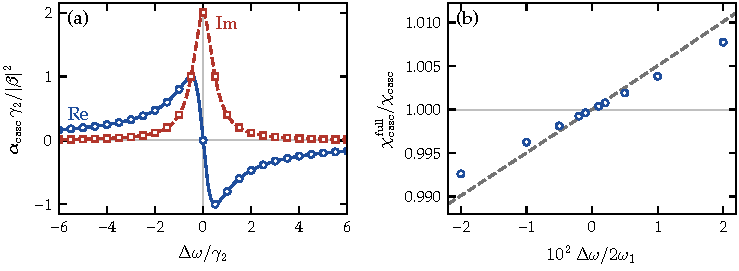
\includegraphics[width=\linewidth]{figures/fig_s1_checks.pdf}
  \caption{(a)~Real (solid line, circles) and imaginary (dashed line,
    squares) parts of the cascaded coefficient $\acasc$ of the pump mode,
    in units of $|\beta|^2/\gamma_2$ with $N_1=N_2$, from steady-state
    integration of the two-mode equations (markers) and from
    Eq.~\eqref{eq:acasc} (lines) versus $\Dom/\gamma_2$, for
    $\gamma_1=10\gamma_2$, $\gamma_1^{\mathrm e}=\gamma_1/2$, $\delta_1=0$,
    $\alpha_3=0$ and a drive $|s|^2=10^{-4}\gamma_2^3/|\beta|^2$.
    (b)~Cascaded susceptibility of the two-layer Bloch cell of Section~3
    (indices 2.2 and 1.45, nonlinear layer $0.45\Lambda$, Bloch
    wavevector $0.37\pi/\Lambda$, 1200 grid points per period) from the
    full driven second-harmonic field (circles), divided by
    Eq.~\eqref{eq:chicasc}, versus $\Dom/2\omega_1$.  The dashed line is the
    single-mode pole without linearisation, $1/(1-\Dom/4\omega_1)$.}
  \label{fig:s-checks}
\end{figure}

\section{Response time, loss and thresholds}

\subsection{Response to a modulated pump}

Integrating Eq.~(2) of the main text without the steady-state assumption
gives
\begin{equation}
  a_2(t)=i\beta\int_{-\infty}^{t}e^{(i\Dom-\gamma_2/2)(t-t')}a_1^2(t')\,dt' .
\end{equation}
For $a_1^2(t)=\int\tilde A(\Omega)e^{-i\Omega t}d\Omega$, so that $\Omega$
is measured from $2\omega_1$, this is
$a_2=-\beta\int\tilde A(\Omega)e^{-i\Omega t}/(\Dom+\Omega+i\gamma_2/2)\,d\Omega$.
Each component $\tilde A(\Omega)$ of $a_1^2$ therefore enters Eq.~(1) of
the main text with the cascaded susceptibility
\begin{equation}
  \chicasc(\Omega)=-\frac{C}{\Dom+\Omega+i\gamma_2/2},\qquad
  C=\frac{2\omega_1|\chitwo|^2\etag}{3n_2^2}.
  \label{eq:response}
\end{equation}
A real modulation of the pump intensity at frequency $\Omega$ contains both
components $\pm\Omega$ and samples $\chicasc(\pm\Omega)$.  The response has
a single pole at $\Omega=-\Dom-i\gamma_2/2$, in the lower half-plane, and
for any $Q_2$ and $\Dom$ it obeys
\begin{equation}
  |\chicasc(0)|\,|\Dom+i\gamma_2/2|=C,\qquad
  \int_{-\infty}^{\infty}\mathrm{Im}\,\chicasc(\Omega)\,d\Omega=\pi C .
  \label{eq:sum}
\end{equation}
The first relation fixes the product of the static susceptibility and the
distance of the pole from the origin, which limits the quasi-static
bandwidth.  The second, a sum rule over the modulation frequency, states
that the integrated nonlinear absorption does not depend on the
linewidth.  With
$\Delta f\le|\Dom+i\gamma_2/2|/2\pi$ the first relation gives Eq.~(5) of
the main text.  At $\Dom=2\gamma_2$, $|\chicasc(\Omega)/\chicasc(0)|$ lies
between 0.81 and 1.30 for $|\Omega|\le\gamma_2/2$.

\subsection{Nonlinear loss and stability}

From Eq.~\eqref{eq:chicasc},
$\mathrm{Im}\,\chicasc/\mathrm{Re}\,\chicasc=-\gamma_2/(2\Dom)$, so the
loss-to-Kerr ratio of the cascade is $\rho=\gamma_2/(2|\Dom|)$.  The
second-harmonic energy is $W_2=2N_2|a_2|^2$, and
\begin{equation}
  \frac{W_2}{W_1}=\frac{|\acasc|\,|a_1|^2}{|\Dom+i\gamma_2/2|}.
\end{equation}
This ratio equals $S/|\Dom|$, where $S=|\mathrm{Re}\,\acasc||a_1|^2$ is the
cascaded shift of the pump resonance.  In a continuous-wave steady state
the elimination of $a_2$ is exact at any power, and $\mathrm{Im}\,\acasc$
accounts for the power transferred to the second harmonic.  The steady
state can, however, lose stability through a Hopf bifurcation to
self-pulsing, as in doubly resonant second-harmonic
generation~\cite{drummond1980}.  In the two-mode equations this happens once
$S$ exceeds $|\Dom|$ by a factor that depends on $\gamma_1$ and $\delta_1$.
The factor is about 1.1 for the microring of Section~8 and 2.9 for
$\gamma_1=10\gamma_2$, both at $\delta_1=0$, and reaches about 10 at large
pump detuning.

Equations~(1) and (2) of the main text keep only the native self-phase
modulation of the pump, which shifts its resonance by
$\alpha_3|a_1|^2=S/R$, with $R=|\mathrm{Re}\,\acasc|/\alpha_3$ as in Eq.~(6)
of the main text.  For a
field that is uniform in the second-order material, the native
cross-phase modulation, with the factor 6 of Ref.~\cite{boyd2020}, shifts
the second-harmonic mode by about $4S/R$ and the pump mode by about
$2S^2/(R|\Dom|)$, and the native self-phase modulation of the second
harmonic shifts its mode by about $2S^2/(R|\Dom|)$.  The two shifts of the
second-harmonic mode change $\Dom$ and must be small compared with
$|\Dom|$, which requires $S\ll|\Dom|R/4$ and $S\ll|\Dom|(R/2)^{1/2}$; for
$R\gtrsim8$ the second condition is the stricter.  For $S<2|\Dom|$ the
cross-phase term is the larger of the two; at the folds of Fig.~3(c) of the
main text, where $S$ is $0.46|\Dom|$ and $0.78|\Dom|$ and $R=20$, it amounts
to at most $0.16|\Dom|$.

\subsection{Bistability}

Write the total Kerr coefficient $\alpha_3+\acasc$ as $\alpha=\alpha'+i\alpha''$
with $\alpha''\ge0$, and let $\rho_{\mathrm{tot}}=\alpha''/|\alpha'|$ and
$y=|a_1|^2$.  Then $\rho_{\mathrm{tot}}=\rho R/|R\mp1|$, with the upper sign for $\Dom>0$,
where the cascaded and native terms have opposite signs; for $R\gg1$,
$\rho_{\mathrm{tot}}\simeq\rho$.  The steady state of Eq.~(1) of the main
text gives
\begin{equation}
  \frac{\gamma_1^{\mathrm e}}{2N_1}|s|^2=y\bigl[(\delta_1+\alpha'y)^2+(\gamma_1/2+\alpha''y)^2\bigr],
\end{equation}
and the response is bistable when $d|s|^2/dy<0$ for some $y>0$.  The
derivative is the quadratic
$3|\alpha|^2y^2+4(\alpha'\delta_1+\alpha''\gamma_1/2)y+\delta_1^2+\gamma_1^2/4$,
which has positive roots only if the vectors $(\alpha',\alpha'')$ and
$(\delta_1,\gamma_1/2)$ make an angle larger than $150^\circ$.  The first
vector makes an angle $\arctan\rho_{\mathrm{tot}}$ with the $\alpha'$ axis
and the second lies in the upper half-plane, so bistability is possible
only for $\arctan\rho_{\mathrm{tot}}<30^\circ$, that is
$\rho_{\mathrm{tot}}<1/\sqrt3$.  It then requires a pump detuning of the
opposite sign to $\alpha'$ with
\begin{equation}
  \frac{2|\delta_1|}{\gamma_1}>\cot\bigl(30^\circ-\arctan\rho_{\mathrm{tot}}\bigr),
\end{equation}
which is $\sqrt3$ for $\rho_{\mathrm{tot}}=0$ and 3.50 for
$\rho_{\mathrm{tot}}=1/4$.  Since $\Dom$ is defined with the pump
frequency, the resonator must be designed with the cold mismatch
$2\omega_a-\omega_2=\Dom-2\delta_1$.

We take as the bistability threshold the input power at which the lower
branch switches up, the larger of the two fold powers, minimised over
$\delta_1$.  Because the cascaded loss raises the required detuning, the
threshold falls by less than the Kerr coefficient.  With
$\alpha_3=|\mathrm{Re}\,\acasc|/R$ and $\Dom=-2\gamma_2$, so that the
cascaded and native terms add and $\rho=1/4$, the threshold with the
cascade is lower than that of the native response alone by a factor
$(1+R)/4.7$ for
$R=10$, $(1+R)/5.2$ for $R=20$ and $(1+R)/5.8$ for $R\to\infty$.  The last
value is the ratio of the thresholds of a lossless Kerr term and of one
with $\rho_{\mathrm{tot}}=1/4$.

\subsection{Parametric gain}

In a resonator with several pump-band modes, a pair of sidebands $a_\pm$
at frequencies $\omega_1\pm\nu$, in modes detuned from them by
$\delta_\pm$, obeys in the effective Kerr description
\begin{equation}
  \dot a_\pm=\bigl(i\delta_\pm-\tfrac{\gamma_1}{2}+2i\alpha y\bigr)a_\pm
  +i\alpha a_1^2a_\mp^* .
\end{equation}
For symmetric detunings the largest growth rate, reached when
$\delta_\pm+2\alpha'y=0$, is $(|\alpha|-2\alpha'')y-\gamma_1/2$.  Gain is
possible only if $|\alpha|>2\alpha''$, which is again
$\rho_{\mathrm{tot}}<1/\sqrt3$, and the threshold is
$y=\gamma_1/[2|\alpha'|(\sqrt{1+\rho_{\mathrm{tot}}^2}-2\rho_{\mathrm{tot}})]$.
With a single second-harmonic mode the cross terms of the sidebands carry
the cascaded coefficient at $\Dom\pm\nu$, so this description requires
$|\nu|\ll|\Dom+i\gamma_2/2|$.  In a multimode resonator the cross terms
couple the sidebands through other second-harmonic modes, and the
threshold must be computed with those modes included (Section~8).

\section{Host materials}

At $\Dom=2\gamma_2$ and with $\gamma_2=\omega_2/Q_2\simeq2\omega_1/Q_2$,
Eq.~\eqref{eq:chicasc} gives
\begin{equation}
  R=\frac{|\mathrm{Re}\,\chicasc|}{\chinat}
  =\frac{Q_2\etag F}{6}\cdot\frac{1}{1+(\gamma_2/2\Dom)^2}
  =\frac{Q_2\etag F}{6.375},\qquad F=\frac{|\chitwo|^2}{n_2^2\chinat}.
\end{equation}
The main text quotes the approximation $Q_2\etag F/6$, and $R=1$ at
$Q_2=6/(\etag F)$.

Table~\ref{tab:s-hosts} lists the constants for a pump at 1.55~\textmu m.
The second-order coefficients are scaled to this wavelength with Miller's
rule~\cite{miller1964}.  For congruent LiNbO$_3$ we start from $d_{33}=19.5$~pm/V at
1.313~\textmu m~\cite{shoji1997}, and for bulk AlN from $d_{33}=4.3$~pm/V
at 1.03~\textmu m~\cite{majkic2017}.  For GaP the starting value is
$d_{14}=70.6$~pm/V at 1.064~\textmu m~\cite{shoji1997}; its second
harmonic lies above the indirect gap, so the scaled value is an upper
estimate.  For Al$_{0.2}$Ga$_{0.8}$As we use the ratio
$d_{14}/d_{33}=5.01$ of GaAs to LiNbO$_3$ at 4.1~\textmu m~\cite{skauli2002}
and scale it in wavelength and composition, which gives
$d_{14}=92.6$~pm/V.  The refractive indices
are from Refs.~\cite{zelmon1997,bond1965,pastrnak1966,gehrsitz2000}; the
pump and the second harmonic are extraordinary in LiNbO$_3$ and AlN, and
$n_2$, the smallest principal index at $2\omega_1$, is $n_e$ for LiNbO$_3$
and $n_o$ for AlN.  The native Kerr indices are
$n_2^I=1.8\times10^{-19}$~m$^2$/W for LiNbO$_3$, the value used for
microresonators~\cite{kovach2020}, $1.1\times10^{-17}$~m$^2$/W for
GaP~\cite{wilson2020}, $3.5\times10^{-19}$~m$^2$/W for AlN~\cite{liu2018}
and $2.6\times10^{-17}$~m$^2$/W for AlGaAs~\cite{pu2016}.  They are
converted with $\chinat=4\varepsilon_0cn_1^2n_2^I/3$, where $n_1$ is the
index at the pump.

The native index of LiNbO$_3$ is the least certain input.  The value
above was inferred from the parametric-oscillation threshold of a
microring with ordinary polarisation~\cite{he2019}.  Cross-phase
modulation in a thin-film ring at 1550~nm gives
$1.74\times10^{-19}$~m$^2$/W for extraordinary and
$1.61\times10^{-19}$~m$^2$/W for ordinary polarisation, with a cascaded
contribution of opposite sign estimated below 10\% and not
subtracted~\cite{shamsansari2022}.  A Z-scan at
1.064~\textmu m gives $0.91\times10^{-19}$~m$^2$/W~\cite{desalvo1996}, a
value that contains the negative cascaded contribution of the bulk
crystal; without that contribution the index is
$3.9\times10^{-19}$~m$^2$/W~\cite{phillips2011,bache2012}.  Equation
\eqref{eq:bulk} accounts for the difference: with $d_{33}=25.2$~pm/V at
1.064~\textmu m~\cite{shoji1997} and the extraordinary indices of
Ref.~\cite{zelmon1997}, the bulk cascade contributes
$-3.0\times10^{-19}$~m$^2$/W, and the sum with $3.9\times10^{-19}$~m$^2$/W
is $0.89\times10^{-19}$~m$^2$/W.  With the two-band
dispersion of Ref.~\cite{sheikbahae1991} we estimate about
$3.2\times10^{-19}$~m$^2$/W at 1.55~\textmu m.  For $n_2^I$ between 1.8
and $3.2\times10^{-19}$~m$^2$/W and $d_{33}$ between 18.8 and 22.7~pm/V
(Miller's rule from the two wavelengths of Ref.~\cite{shoji1997}), $R$ of
LiNbO$_3$ at $Q_2=4000$ and $\etag=0.3$ lies between 11 and 30.  For GaP, AlN and AlGaAs the reported spreads give $F$
between $2\times10^{-3}$ and $9\times10^{-3}$, so the three cannot be ranked
against one another.  Their absorption differs.  AlN absorbs at
neither wavelength, and GaP has two-photon absorption at the second
harmonic~\cite{vermeulen2023}.  The second harmonic of
Al$_{0.2}$Ga$_{0.8}$As lies 74~meV below the band gap of
1.67~eV~\cite{adachi1985}, where the absorption tail adds loss, and the
two-photon absorption of one pump and one second-harmonic photon, with
$0.8+1.6$~eV above the gap, adds a pump loss that grows with the
second-harmonic intensity.  GaAs is not
listed because its second harmonic at 775~nm lies above the band gap.

\begin{table}[htbp]
  \centering
  \caption{\bf Host Constants for a Pump at 1.55~\textmu m and the Ratio $R=Q_2\etag F/6$ at $Q_2=4000$, $\Dom=2\gamma_2$ and $\etag=0.3$}
  \label{tab:s-hosts}
  \small
  \setlength{\tabcolsep}{4pt}
  \begin{tabular}{lcccccccc}
    \toprule
    Host & $|\chitwo|$ (pm/V) & $n_1$ & $n_2$ & $n_2^I$ (m$^2$/W) & $\chinat$ (m$^2$/V$^2$) & $F$ & $R$ & $Q_2$ at $R=1$\\
    \midrule
    LiNbO$_3$ & 37.5 & 2.14 & 2.18 & $1.8\times10^{-19}$ & $2.9\times10^{-21}$ & 0.10   & 20   & 200 \\
    GaP       & 130  & 3.05 & 3.20 & $1.1\times10^{-17}$ & $3.6\times10^{-19}$ & 0.0045 & 0.91 & $4.4\times10^3$ \\
    AlN       & 8.1  & 2.16 & 2.14 & $3.5\times10^{-19}$ & $5.8\times10^{-21}$ & 0.0025 & 0.49 & $8.1\times10^3$ \\
    Al$_{0.2}$Ga$_{0.8}$As & 214 & 3.27 & 3.53 & $2.6\times10^{-17}$ & $9.8\times10^{-19}$ & 0.0037 & 0.75 & $5.4\times10^3$ \\
    \bottomrule
  \end{tabular}
\end{table}

\section{Coupled-mode simulations}

Equations, integrator, tolerances, run lengths and convergence criterion
for Figs.~3 and 4 of the main text and Fig.~\ref{fig:s-checks}, and the
time-domain model for pulsed excitation used in Fig.~4(d) of the main
text.

\section{Singly resonant metasurface}

Without a pump resonance the pump field in the structure is
$E_{\mathrm{in}}\mathbf e_1(\mathbf r)$, with $E_{\mathrm{in}}$ the incident
amplitude and $\mathbf e_1$ the linear field per unit incident amplitude.
Equation~(\ref{eq:projection}) for the second-harmonic mode gives, in
steady state,
\begin{equation}
  a_2=-\frac{\varepsilon_0\omega_1\widetilde M E_{\mathrm{in}}^2}{N_2(\Dom+i\gamma_2/2)},\qquad
  \widetilde M=\int\chitwo_{ijk}f^*_{2,i}e_{1,j}e_{1,k}\,d^3r .
\end{equation}
The projections of the cascaded and native polarisations onto
$\mathbf e_1^*$ are
\begin{equation}
  -\frac{2\varepsilon_0^2\omega_1|\widetilde M|^2}{N_2(\Dom+i\gamma_2/2)}\,|E_{\mathrm{in}}|^2E_{\mathrm{in}}
  \quad\text{and}\quad
  3\varepsilon_0\chinat|E_{\mathrm{in}}|^2E_{\mathrm{in}}\int_{\NL}|\mathbf e_1|^4d^3r .
\end{equation}
By reciprocity, the field that a nonlinear polarisation $\delta\mathbf P$
radiates into the transmitted wave is proportional to
$\int\mathbf e_1^{\mathrm{rec}}\cdot\delta\mathbf P\,d^3r$, where
$\mathbf e_1^{\mathrm{rec}}$ is the linear field excited by a wave incident
from the detection side~\cite{obrien2015}.  The projections above set the
measured cascaded and native phases when $\mathbf e_1^{\mathrm{rec}}$ is
proportional to $\mathbf e_1^*$ in the second-order material, as for a
film much thinner than the wavelength and symmetric under reflection
through its mid-plane, in which $\mathbf e_1$ has a uniform phase.  A
substrate breaks this symmetry; then one factor $\widetilde M^*$ of the
cascaded projection and one factor $\mathbf e_1^*$ of the native projection
are replaced by the corresponding integrals with $\mathbf e_1^{\mathrm{rec}}$.
If the transmitted field has a phase relative to $\mathbf e_1$, the real and
imaginary parts of the cascaded response mix in that phase.  The ratio of
the real parts is
\begin{equation}
  R^{(1)}=\frac{2\omega_1|\chitwo|^2\eta^{(1)}}{3n_2^2\chinat}\,
  \frac{|\Dom|}{\Dom^2+(\gamma_2/2)^2},\qquad
  \eta^{(1)}=\frac{\varepsilon_0n_2^2|\widetilde M|^2}{|\chitwo|^2N_2\int_{\NL}|\mathbf e_1|^4d^3r}\le1,
\end{equation}
which reduces at $\Dom=2\gamma_2$ to Eq.~(6) of the main text with $\etag$
replaced by $\eta^{(1)}$.  The local field enhancement enters $\widetilde M$ and
$\int_{\NL}|\mathbf e_1|^4$ alike and cancels in $R^{(1)}$; it enters the
nonlinear phase per unit incident power.

For a given design, $\eta^{(1)}$ follows from two full-wave calculations
of the unit cell with periodic boundary conditions.  An eigenfrequency
calculation near $2\omega_1$ gives the second-harmonic mode $\f_2$, its
quality factor $Q_2=\omega_2/\gamma_2$ and $N_2$ from Eq.~\eqref{eq:Nn}.  A
frequency-domain calculation at $\omega_1$ with a normally incident plane
wave of unit amplitude gives $\mathbf e_1$.  The overlap $\widetilde M$
and $\int_{\NL}|\mathbf e_1|^4d^3r$ are then integrated over the
second-order material, with the tensor of Eq.~\eqref{eq:pol} rotated to the
crystal orientation of the film.  Since $\eta^{(1)}$ does not depend on the
normalisation of $\f_2$ or on the incident amplitude, neither has to be
fixed in the simulations.
% FOR THE DESIGN (Sedigheh): geometry, materials and crystal orientation;
% Q2, omega2, M-tilde, eta^(1) and R^(1) at Domega = +-2 gamma2 from the recipe
% above; then the Z-scan model (pulse length, beam waist, the odd part in
% Domega at fixed pump detuning) used for Fig. 4 of the main text.

The parameters of the design and the Z-scan model.

\section{Microring}

\subsection{Photon-number form}

The $\chitwo$ microresonator literature uses photon-number amplitudes.
With $\hat a=a_1(2N_1/\hbar\omega_1)^{1/2}$ and
$\hat b=a_2(N_2/\hbar\omega_1)^{1/2}$, so that $|\hat a|^2$ and
$|\hat b|^2$ are the photon numbers of the pump and second-harmonic modes,
Eqs.~(1) and (2) of the main text become
\begin{align}
  \dot{\hat a}&=(i\delta_1-\kappa_1)\hat a-2ig\,\hat a^*\hat b+iU_{\mathrm{nat}}|\hat a|^2\hat a+\sqrt{2\kappa_1^{\mathrm e}}\,s_{\mathrm{in}},
  \label{eq:ring-a}\\
  \dot{\hat b}&=(i\Dom-\kappa_2)\hat b-ig\,\hat a^2 ,
  \label{eq:ring-b}
\end{align}
where $\kappa_n=\gamma_n/2$ are amplitude decay rates, $\kappa_1^{\mathrm e}=\gamma_1^{\mathrm e}/2$
refers to the bus waveguide, $|s_{\mathrm{in}}|^2$ is the
incident photon flux, and the phase of $\hat b$ is chosen to make $g$ real.
The coupling rate is
\begin{equation}
  g=\frac{\varepsilon_0\omega_1|M|}{2N_1N_2^{1/2}}\,(\hbar\omega_1)^{1/2},
  \label{eq:g}
\end{equation}
which is the standard rate
\begin{equation*}
  \Bigl(\frac{\hbar\omega_1^2\omega_2}{8\varepsilon_0}\Bigr)^{1/2}
  \frac{\bigl|\int\chitwo_{ijk}E_{1,i}E_{1,j}E^*_{2,k}\,d^3r\bigr|}
       {\int\varepsilon_r|\mathbf E_1|^2d^3r\,\bigl(\int\varepsilon_r|\mathbf E_2|^2d^3r\bigr)^{1/2}}
\end{equation*}
of the Hamiltonian $\hat H/\hbar=g[(\hat a^\dagger)^2\hat b+\hat a^2\hat b^\dagger]$
for a nondispersive resonator~\cite{zhao2022,lu2020}.  The native Kerr
shift per photon is $U_{\mathrm{nat}}=\alpha_3\hbar\omega_1/2N_1$.  For a
ring of radius $R_{\mathrm{ring}}$ and mode area $A_{\mathrm{eff}}$, the
round-trip Kerr phase gives
\begin{equation}
  U_{\mathrm{nat}}=\frac{\hbar\omega_1^2cn_2^I}{n_{g1}^2V_{\mathrm{eff}}},\qquad
  V_{\mathrm{eff}}=2\pi R_{\mathrm{ring}}A_{\mathrm{eff}},
  \label{eq:Unat}
\end{equation}
with $n_{g1}$ the group index at the pump.

\subsection{Cascaded Kerr coefficient and the coupling rate}

The steady state of Eq.~\eqref{eq:ring-b},
$\hat b=-ig\hat a^2/(\kappa_2-i\Dom)$, turns the coupling term of
Eq.~\eqref{eq:ring-a} into $(iU_{\mathrm{casc}}-\kappa_{\mathrm{casc}})|\hat a|^2\hat a$
with
\begin{equation}
  U_{\mathrm{casc}}=-\frac{2g^2\Dom}{\Dom^2+\kappa_2^2},\qquad
  \kappa_{\mathrm{casc}}=\frac{2g^2\kappa_2}{\Dom^2+\kappa_2^2},
  \label{eq:Ucasc}
\end{equation}
the photon-number form of Eq.~\eqref{eq:acasc}.  The pump resonance moves to
$\omega_a-(U_{\mathrm{nat}}+U_{\mathrm{casc}})|\hat a|^2$, and
$R=|U_{\mathrm{casc}}|/U_{\mathrm{nat}}$.  Since $g^2$ and
$U_{\mathrm{nat}}$ both scale as $1/V_{\mathrm{eff}}$, $R$ does not depend on
the size of the ring, and $R\propto Q_2$ at fixed $\Dom/\gamma_2$.  These
expressions describe the cascaded Kerr response measured in AlN
microrings~\cite{cui2022,cui2025}.

The coupling rate follows from the second-harmonic efficiency.  On double
resonance and for an undepleted pump,
Eqs.~(\ref{eq:ring-a}) and (\ref{eq:ring-b}) give
\begin{equation}
  \eta_{\mathrm{SHG}}=\frac{P_{\mathrm{SH}}}{P_{\mathrm{in}}^2}
  =\frac{16g^2\kappa_2^{\mathrm e}(\kappa_1^{\mathrm e})^2}{\hbar\omega_1\kappa_2^2\kappa_1^4},
  \label{eq:etashg}
\end{equation}
with $P_{\mathrm{in}}$ the pump power in the bus waveguide,
$P_{\mathrm{SH}}$ the second-harmonic power coupled out of the ring and
$\kappa_2^{\mathrm e}$ the out-coupling rate of the second harmonic.  This
is Eq.~(4) of Ref.~\cite{lu2020} at zero detuning, and Eq.~\eqref{eq:g} follows
Ref.~\cite{lu2019}.

\subsection{Cascaded shift from measured quantities}

The pump loses energy to the second-harmonic mode at the rate
$2\kappa_{\mathrm{casc}}|\hat a|^2$, so
$\kappa_{\mathrm{casc}}|\hat a|^2=P_{\mathrm{SH}}^{\mathrm{tot}}/2W_1$, where
$W_1=\hbar\omega_1|\hat a|^2$ is the energy stored in the pump mode and
$P_{\mathrm{SH}}^{\mathrm{tot}}=(\kappa_2/\kappa_2^{\mathrm e})P_{\mathrm{SH}}$
is the total second-harmonic power generated, of which $P_{\mathrm{SH}}$
leaves through the bus.  With $-U_{\mathrm{casc}}/\kappa_{\mathrm{casc}}=\Dom/\kappa_2$
from Eq.~\eqref{eq:Ucasc}, the cascaded shift of the pump resonance is
\begin{equation}
  \delta\omega_{\mathrm{casc}}=-U_{\mathrm{casc}}|\hat a|^2
  =\frac{\Dom}{\kappa_2}\,\frac{P_{\mathrm{SH}}^{\mathrm{tot}}}{2W_1}.
  \label{eq:shift-energy}
\end{equation}
This relation holds at any pump detuning and power within the
elimination, and the same argument applied to Eq.~\eqref{eq:acasc} gives it
for any resonator.  For a pump locked to its resonance and with the
nonlinear loss neglected,
$W_1=2\kappa_1^{\mathrm e}P_{\mathrm{in}}/\kappa_1^2$ and
$P_{\mathrm{SH}}=\eta_{\mathrm{SHG}}P_{\mathrm{in}}^2\kappa_2^2/(\Dom^2+\kappa_2^2)$
from Eq.~\eqref{eq:etashg}, so
\begin{equation}
  \frac{\delta\omega_{\mathrm{casc}}}{\kappa_1}
  =\frac{\eta_{\mathrm{SHG}}P_{\mathrm{in}}}{4}\,
  \frac{\kappa_1}{\kappa_1^{\mathrm e}}\,\frac{\kappa_2}{\kappa_2^{\mathrm e}}\,
  \frac{\kappa_2\Dom}{\Dom^2+\kappa_2^2},
  \label{eq:shift-eta}
\end{equation}
which is Eq.~(7) of the main text at critical coupling,
$\kappa_n^{\mathrm e}=\kappa_n/2$.  The coupling ratios follow from the
loaded and intrinsic quality factors,
$\kappa_n^{\mathrm e}/\kappa_n=1-Q_n^{\mathrm{load}}/Q_n^{\mathrm{int}}$.  For
the device of Ref.~\cite{lu2020} they are 0.70 and 0.22, the product of the
coupling factors in Eq.~\eqref{eq:shift-eta} is 1.59, and
$\eta_{\mathrm{SHG}}=5\times10^6$\%/W gives
$\delta\omega_{\mathrm{casc}}/\kappa_1=0.094$ at $P_{\mathrm{in}}=5$~\textmu W
and $\Dom=2\gamma_2$.  With the pump locked, the nonlinear loss lowers the
photon number by the factor
$(1+\kappa_{\mathrm{casc}}|\hat a|^2/\kappa_1)^{-2}$, which is 0.96 at this
point and 0.76 at $|\Dom|=\kappa_2$, where $\rho=1$ [main text,
Fig.~5(b)].  Measuring $P_{\mathrm{SH}}$ and $W_1$ at the operating point and
using Eq.~\eqref{eq:shift-energy} would avoid this correction.

\subsection{Design points}

Of the three designs in Table~\ref{tab:s-rings}, design A is the
periodically poled ring of Ref.~\cite{lu2020}, with the coupling rate obtained there
from a fit of the measured lineshape.  Design B applies the same poling to
a ring with a higher pump quality factor; its $g$ is scaled from A as
$V_{\mathrm{eff}}^{-1/2}$.  Design C is ring B without poling,
phase matched through mode order or the cyclic crystal orientation, for
which we take $g$ 12 times smaller, an estimate for an interaction through
$d_{31}$ with a mismatched transverse mode.  For design A, Eq.~\eqref{eq:etashg} with the
efficiency reported in Ref.~\cite{lu2020} gives $g/2\pi=0.56$~MHz instead
of the fitted 1.2~MHz, which would lower its $R$ to about 600; the fit
may include a residual second-harmonic detuning that Eq.~\eqref{eq:etashg}
omits.  Since $U_{\mathrm{nat}}$ uses the assumed $A_{\mathrm{eff}}$ while $g$
is measured, $R$ of design A also scales with $A_{\mathrm{eff}}$.

\begin{table}[htbp]
  \centering
  \caption{\bf Microring Designs and Cascaded Response at $\Dom=2\gamma_2$}
  \label{tab:s-rings}
  \footnotesize
  \setlength{\tabcolsep}{3pt}
  \begin{tabular}{lccccccccc}
    \toprule
    Design & $Q_1$ & $Q_2$ & $R_{\mathrm{ring}}$ (\textmu m) & $g/2\pi$ (MHz) & $R$ & $U/2\pi$ (Hz) & $P_{\mathrm{bist}}$ (\textmu W) & $P_{\mathrm{par}}$ (\textmu W)\\
    \midrule
    A, poled~\cite{lu2020} & $5.4\times10^5$ & $4.5\times10^5$ & 70 & 1.20 & 2800 & $-1590$ & 73 & 19 \\
    B, poled & $1.0\times10^6$ & $3.0\times10^5$ & 50 & 1.42 & 1830 & $-1470$ & 37 & 8.0 \\
    C, not poled & $1.0\times10^6$ & $3.0\times10^5$ & 50 & 0.12 & 13 & $-10$ & 7000 & 1150 \\
    B, native only & $1.0\times10^6$ & -- & 50 & -- & -- & $+0.80$ & 14400 & 9400 \\
    \bottomrule
  \end{tabular}

  \smallskip
  \footnotesize Loaded quality factors; the intrinsic values are
  $1.8\times10^6$ and $5.8\times10^5$ for A and $2\times10^6$ and
  $6\times10^5$ for B and C.  Pump wavelength 1.56~\textmu m (A) and
  1.55~\textmu m (B, C); $A_{\mathrm{eff}}=1$~\textmu m$^2$, $n_{g1}=2.30$,
  $n_{g2}=2.45$, $n_2^I=1.8\times10^{-19}$~m$^2$/W.  $U$ is $U_{\mathrm{casc}}$,
  or $U_{\mathrm{nat}}$ in the native row.  $P_{\mathrm{bist}}$ and
  $P_{\mathrm{par}}$ are input powers at the bistability and parametric
  thresholds of Sections~8.E and 8.F, for a cold mismatch of $2\gamma_2$ and
  a second-order dispersion $D_2/2\pi=10$~MHz.
\end{table}

\subsection{Bistability}

The steady state of Eq.~\eqref{eq:ring-a} with the cascaded terms is the cubic
of Section~4.C in photon units, with $\alpha'\to U_{\mathrm{nat}}+U_{\mathrm{casc}}$,
$\alpha''\to\kappa_{\mathrm{casc}}$, $\gamma_1/2\to\kappa_1$ and the drive
$2\kappa_1^{\mathrm e}|s_{\mathrm{in}}|^2$.  In a ring the pump
detuning needed for bistability, a few $\kappa_1$, changes $\Dom$ by an
amount comparable with $\kappa_2$, because $\Dom=\Dom_0+2\delta_1$ with
$\Dom_0=2\omega_a-\omega_2$ fixed by the device.  The threshold is
therefore found by minimising the fold power over $\delta_1$ with
$U_{\mathrm{casc}}$ and $\kappa_{\mathrm{casc}}$ evaluated at $\Dom_0+2\delta_1$.
The condition $\rho<1/\sqrt3$ of Section~4.C then applies to the
pump-frame $\Dom$ and does not restrict $\Dom_0$.  For design B the
threshold is 37~\textmu W at $\Dom_0=2\gamma_2$ and has a shallow minimum
of 32~\textmu W at $\Dom_0=3.3\gamma_2$, against 14.4~mW for the native
response of this ring.  These are the folds of the single-mode cubic.
In a multimode ring the parametric threshold of Section~8.F lies below
them, for the cascaded and the native response alike, so the upper branch
carries parametric sidebands unless the dispersion suppresses them.  A
shift of the pump resonance by its half-width $\kappa_1$ needs
$\kappa_1/|U_{\mathrm{nat}}+U_{\mathrm{casc}}|=6.6\times10^4$ photons in
design B, an intracavity energy of 8.4~fJ, against 15~pJ for the native
response.

The steady state of the two-mode equations stays stable up to a cascaded
shift of about $1.1|\Dom|$.  For design B at $\Dom=2\gamma_2$ and
$\delta_1=0$, the largest real part of the eigenvalues of the
four-dimensional Jacobian of
Eqs.~(\ref{eq:ring-a}) and (\ref{eq:ring-b}) crosses zero at
$2.0\times10^6$ photons, a cascaded shift of $30\kappa_1$.  This photon
number is 1.1 times $(\Dom^2+\kappa_2^2)/2g^2$, the value at which
$|U_{\mathrm{casc}}||\hat a|^2=|\Dom|$.

\subsection{Parametric gain}

The degenerate four-wave mixing that produces parametric gain is mediated
by the same second-harmonic mode $b_0$ as the pump self-phase modulation,
while the cross-phase terms of the sidebands pass through the
second-harmonic modes $b_\pm$ at azimuthal orders $2m_p\pm q$.  With the
pump $a_0$ at order $m_p$ and the sidebands $a_\pm$ at $m_p\pm q$, the
relevant part of the Hamiltonian is
\begin{equation}
  \hat H/\hbar\supset g\,\hat a_0^{\dagger2}\hat b_0
  +2g\,\hat a_+^\dagger\hat a_-^\dagger\hat b_0
  +2g\,\hat a_0^\dagger\hat a_+^\dagger\hat b_+
  +2g\,\hat a_0^\dagger\hat a_-^\dagger\hat b_-+\mathrm{h.c.},
\end{equation}
assuming equal overlaps for all triplets.  Linearising about the pump
gives a four-dimensional system for
$(\delta\hat a_+,\delta\hat a_-^*,\delta\hat b_+,\delta\hat b_-^*)$, and the
threshold is the lowest input power at which an eigenvalue acquires a
positive real part, minimised over $\delta_1$ and $q$.  The modes $b_\pm$
are detuned from $b_0$ by $\pm q(D_1^{(2)}-D_1^{(1)})$, where
$D_1^{(n)}$ is the free spectral range of band $n$ in angular units and
$D_1^{(2)}-D_1^{(1)}=D_1^{(1)}(n_{g1}/n_{g2}-1)$, $-2\pi\times25$~GHz or
$-20\gamma_2$ per azimuthal order for design B.  The sidebands are detuned
from the pump-band modes by the integrated dispersion $D_2q^2/2$, with
$D_2$ the second-order dispersion parameter.  Without
the walk-off of the second-harmonic modes the system reduces to the
single-pair result of Section~4.D.  For design B the threshold is
8.0~\textmu W, with a spread below 2\% for anomalous dispersion
$D_2/2\pi$ between 1 and 50~MHz, and 11.6~\textmu W for normal dispersion,
$D_2/2\pi=-10$~MHz, against 9.4~mW for the native response.

\subsection{Response time}

In a ring $\gamma_2/\gamma_1=2Q_1/Q_2$, which is 6.7 for design B, so the
second-harmonic mode responds faster than the pump mode.  We compare the
small-signal response of
Eqs.~(\ref{eq:ring-a}) and (\ref{eq:ring-b}) to a modulation of the input power
with that of a single-mode cavity with the same photon number, Kerr
coefficient and nonlinear loss but an instantaneous response.  For design
B at $\Dom=2\gamma_2$, $\delta_1=0$ and 7~\textmu W, below the parametric
threshold, the 3-dB bandwidth is smaller by 4\%, and by 7\% at
20~\textmu W.

\subsection{Thermal and photorefractive shifts}

At the powers of Table~\ref{tab:s-rings}, absorption heats the ring and
shifts the pump resonance to lower frequency.  In a lumped model the shift
is $|d\omega_a/dT|R_{\mathrm{th}}P_{\mathrm{abs}}$, with $R_{\mathrm{th}}$
the thermal resistance of the ring and
\begin{equation}
  P_{\mathrm{abs}}=f_{\mathrm{abs}}\Bigl[2\hbar\omega_1\kappa_{1,0}|\hat a|^2
  +\frac{\kappa_{2,0}}{\kappa_2}\,2\hbar\omega_1\kappa_{\mathrm{casc}}|\hat a|^4\Bigr],
\end{equation}
where $\kappa_{n,0}$ are intrinsic decay rates and $f_{\mathrm{abs}}$ is the
absorbed fraction of the intrinsic loss.  The second term is the power
transferred to the second harmonic, of which the fraction
$\kappa_{2,0}/\kappa_2$ stays on chip.  For design B at 7~\textmu W with
the pump at the cold resonance, $dn/dT=3.3\times10^{-5}$~K$^{-1}$, $R_{\mathrm{th}}=3\times10^4$~K/W and
$f_{\mathrm{abs}}=0.3$, the thermal shift is $1.1\kappa_1$ against a
cascaded shift of $0.7\kappa_1$, in line with the thermal shifts measured in
thin-film LiNbO$_3$ rings~\cite{sun2017}.  The photorefractive effect lowers the
second-harmonic efficiency of poled thin-film rings above about
10~\textmu W~\cite{lu2020} and acts on $\Dom$; it is reduced by removing
the cladding~\cite{xu2021}.

The thermal shift depends on $\Dom$ through $\kappa_{\mathrm{casc}}$, which
is even, and the photorefractive charge generation follows the
second-harmonic intensity, also even to leading order, whereas
$U_{\mathrm{casc}}$ is odd.  To the extent that the backgrounds are even,
the cascaded shift is
\begin{equation}
  \delta\omega^{\mathrm{casc}}(\Dom)=\tfrac12\bigl[\delta\omega(\Dom)-\delta\omega(-\Dom)\bigr]
  \label{eq:antisym}
\end{equation}
under two conditions.  First, the pump must be locked to the resonance as
shifted by all mechanisms.  The photon number then depends on $\Dom$ only
through $\kappa_{\mathrm{casc}}$, which is even, and so do the thermal and
photorefractive shifts.  A pump held at a fixed frequency does not meet
this condition, because
the odd cascaded shift and the even thermal shift detune the cavity
differently for $\pm\Dom$; with the thermal shift of the previous
paragraph, Eq.~\eqref{eq:antisym} then returns less than half of the cascaded
shift.  Second, the zero of the pump-frame $\Dom$ must be referenced in the
same run to the maximum of the second-harmonic power, since an even shift
of the pump frequency or a photorefractive offset of $\Dom$ mixes the odd
and even parts.  Repeating the measurement at two powers would test for a
residual odd background, since the cascaded shift is linear in the photon
number while photorefractive saturation is not.

\subsection{Electro-optic and thermal tuning of \texorpdfstring{$\Dom$}{the mismatch}}

The electro-optic effect shifts each resonance by
$\omega_nn_n^3r_nE_{\mathrm{dc}}/(2n_{gn})$ for a static field
$E_{\mathrm{dc}}$ along the optic axis, so
\begin{equation}
  \frac{d\Dom_0}{dE_{\mathrm{dc}}}=\omega_1\Bigl(\frac{n_1^3r_1}{n_{g1}}-\frac{n_2^3r_2}{n_{g2}}\Bigr)
\end{equation}
for the cold mismatch $\Dom_0$,
with $r_n$ the electro-optic coefficient $r_{33}\approx31$~pm/V~\cite{weis1985}
at each wavelength.  The two terms nearly cancel, so the rate is set by
the dispersion of the indices and of $r_{33}$.  With the extraordinary
indices of Table~\ref{tab:s-hosts}, the group indices of
Table~\ref{tab:s-rings} and equal $r_{33}$ at both wavelengths it is
$+2\pi\times0.2$~GHz per V/\textmu m; an $r_{33}$ larger by 10\% at 775~nm
gives $-2\pi\times2.4$~GHz per V/\textmu m, or $1.8\gamma_2$ for design B.
The rate therefore has to be calibrated on the device.  The pump
resonance itself moves by $2\pi\times13$~GHz per V/\textmu m, about
$130\kappa_1$, so a sweep of $\Dom$ over $\pm2\gamma_2$, which needs
2.2~V/\textmu m peak to peak, requires the pump to follow the resonance.
The difference of the thermo-optic shifts of the two modes also tunes
$\Dom$, by $\gamma_2$ for a change of about 1.4~K in our estimate, with a
magnitude and sign that depend on the dispersion of $dn/dT$ and must be
measured.  An electro-optic dither of $\Dom$ with
lock-in detection and the pump locked to the resonance would extract the
odd part of Eq.~\eqref{eq:antisym} faster than the thermal and photorefractive
responses.

\section{Parameters}

Material constants, mode parameters and design points used in all figures
and tables.

\bibliography{refs}

\end{document}
